Markovketten wurden 1906 von Andrei Andreyvich Markov eingeführt und 
genießen seit jeher große Beliebtheit in vielen Wissenschaftlichen 
Diszpilinen wie Biologie, Sozialwissenschaften, Psychologie und Physik .~\cite{gas}
Das besondere an Markovketten ist, dass sie trotz ihrer simplen Struktur 
in der Lage sind sehr komplexe Prozesse zu modellieren.
Im folgenden werden wir uns auf zeitdiskrete homogene Markovketten beschränken.

Ein zeitdiskreter homogener Markov Prozess modelliert ein zeitdiskretes Signal mit einer endlichen Menge an Zuständen.
Dieser Prozess wird beschrieben durch einen Startwahrscheinlichkeitsvektor $\pi$ und eine Transitionsmatrix $A$.
$\pi_i$ ist die Wahrscheinlichkeit sich in Zeitpunkt $t=0$ in Zustand $S_i$ zu befinden.
$A_{i,j}$ ist die Wahrscheinlichkeit, dass der Prozess sich im nächsten Zeitpunkt in Zustand $S_j$ befindet,
wenn er sich im gegenwärtigen Zeitpunkt im Zustand $S_i$ befindet. In anderen Worten ist $A_{i,j}$ also die Wahrscheinlichkeit einer 
Transition von Zustand $S_i$ nach Zustand $S_j$.
Man beobachte, dass die Transitionswahrscheinlichkeiten unabhängig von $t$ sind, so dass der nächste Zustand 
einzig und allein vom gegenwärtigen Zustand des Prozesses anhängt.
Diese Eigenschaft ist bekannt als Markov-Eigenschaft oder Markov-Bedingung.
Das Ereignis in irgendeinem Zustand zu starten, so wie das Ereignis von einem gegebenen Zustand in irgendeinen anderen Zustand zu wechseln sind sichere Ereignisse.
Somit gelten die Bedingungen, dass die Summe der Startwahscheinlichkeiten $\pi$
und die Summe der ausgehenden Transitionen für jeden Zustand $A_i$ 1 ergeben müssen.

$\sum_{i = 0}^{N} \pi_i = 1 $
$\sum_{j = 0}^{N} A_{i,j} = 1 $

Um das ganze an einem Beispiel zu verdeutlichen stellen wir uns einen Markovprozess vor, welcher 
die durchschnittliche jährliche Temperatur modeliert. Um das Beispiel übersichtlich zu halten beschränken wir uns auf die Zustände Heiß und Kalt.

Die Startwahscheinlichkeiten $\pi$ entsprechen den Wahrscheinlichkeiten, dass ein zufälliger Tag heiß beziehungsweise kalt ist.
Die Transitionswahrscheinlichkeiten seien gegeben durch $A$.
Solch ein Markov Prozess kann anschaulich als gerichteter Transitionsgraph representiert werden.

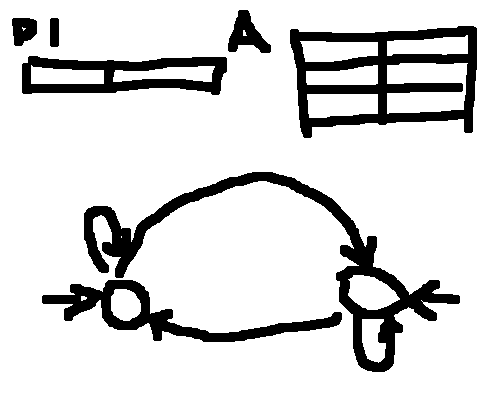
\includegraphics[scale=1.0]{images/Markov_Chain_Example.png}

Mit diesem Modell können wir nun zum Beispiel berechnen, was die Wahrscheinlichkeit ist die Temperaturfolge 
{Heiß, Kalt, Heiß, Kalt, Kalt} zu beobachten unter der Vorraussetzung, dass die gegenwärtige Temperatur Heiß ist.
$O = \{S_1, S_2, S_1, S_2, S_2 \}$
$P(O \mid Model, q_1 = S_1) = P(q_1=S_1 \mid Model) 
\wedge P(S_1 \mid S_1) 
\wedge P(S_2 \mid S_1)
\wedge P(S_1 \mid S_2)
\wedge P(S_2 \mid S_1)
\wedge P(S_2 \mid S_2) $
$= \pi_{1} 
\cdot A_{1,1} 
\cdot A_{1,2} 
\cdot A_{2,1}
\cdot A_{1,2}
\cdot A_{2,2}$
$= 0.8 \cdot 0.4 \cdot 0.3 \cdot 0.7 \cdot 0.5 \cdot 0.3 \cdot 0.9 = 0.009072$

Allgemeiner können wir eine beliebige Observations-Sequenz O berechnen mit 
$O = \{O_1, O_2, \dots, O_{T-1}, O_T \}$
$P(O \mid Model) = \pi_{O_1} \cdot \prod_{t = 2}^{T} A_{O_{t-1}, O_t}$

Mit einer Markovkette können wir jedoch nur Prozesse modellieren welche wir messen können.
Wenn wir einen Prozess $X$ haben den wir nicht beobachten können und einen beobachtbaren Prozess $Y$ welcher von $X$ 
beeinflusst wird, können wir $X$ anhand der von $Y$ generierten Beobachtungen mit einem Hidden Markov Model modellieren.

\section{Hidden Markov Modelle}
Angenommen wir möchten die durchschnittlichen jährlichen Temperaturen 
im Mittelalter modellieren, also für die Jahre 500 bis 1500. In diesem Zeitraum gab es 
noch keine Temperaturaufzeichnungen und wir können die Temperatur somit nicht direkt beobachten.
Es ist jedoch bekannt, dass sich die Temperatur auf das Wachstum von Bäumen auswirkt.
Warme Jahre führen in der Regel zu breiteren Jahresringen und kalte Jahre zu schmaleren.
Die Jahresringe von Bäumen für den gewünschten Zeitraum können wir beobachten.
Seien $\Sigma = \{S, M, L\}$ die Symbole für die verschiedenen Breiten an Jahresringen welche beobachtet werden können.
$S$ steht für dünne, $M$ für mittlere und $L$ für breite Jahresringe.
Unser Modell aus dem vorherigen Abschnitt wird nun um eine Emissionsmatrix $B$ erweitert.
$B_{i, k}$ ist die Wahrscheinlichkeit in Zustand $S_i$ Emissions-Symbol $k$ zu beobachten.
Zum Beispiel gibt $B_{1, 2}$ die Wahrscheinlichkeit an in in einem Heißen Jahr 
Jahresringe mittlerer Breite zu beobachten. Anaolog zu $A$ und $\pi$ sind auch die Reihen von $B$ stochastisch. 
$\sum_{j = 0}^{N} B_{i,j} = 1 $
Die Werte der Parameter $\pi$, $B$ und $A$ gewinnen wir aus den Temperaturaufzeichnungen und Jahresringen der Jahre 1900 bis 2000.

Ein Mögliches Problem welches wir für dieses Hidden Markov Model stellen können ist die Berechnung der Wahrscheinlichkeit
einer Observationssequenz unter einem gegebenen Modell. Zum Beispiel Was ist die Wahrscheinlichkeit 5 aufeinanderfolgende 
Jahre mit dicken Baumringen zu beobachten? Formell formuliert $P({L, L, L, L, L} \mid \lambda)$.
Wenn wir die Abfolge der Zustände $Q={q_1, q_2, q_3, q_4, q_5}$ bereits kennen lässt sich $P(O \mid \lambda)$
sehr einfach berechnen. Die Wahrscheinlichkeit ein Symbol $k$ zu beobachten 
unter der Bedingung in Zustand $S_i$ zu sein ist nichts anderes als $B_{i,k}$
Die Wahrscheilichkeit einer Observationssequenz für ein gegebenes Modell und eine gegebene Abfolge von Zuständen ist also
$P(O \mid Q, \lambda) =  \prod_{t=1}^{T} b_{q_t}(O_t)$
Wenn wir die Abfolge der Zustände jedoch nicht kennen gestaltet sich die Berechnung etwas komplizierter.
Die Wahrscheinlichkeit von $P(O \mid \lambda)$ ist equivalent zu der 
Summe der bedingten Wahrscheinlichkeiten aller möglichen Zustandsfolgen.
$P(O \mid \lambda) = \sum_{all Q} P(O \mid Q, \lambda )$
Es ist möglich $P(O \mid \lambda)$ so zu berechnen, jedoch wächst die 
Anzahl der Möglichen Zustandsabfolgen $Q$ exponentiell in Abhängigkeit von der länge der Observationssequenz $T$.
Präzise gesagt gilt $|Q| = 2T \cdot N^T$. Selbst wenn N und T kleine Werte einnehmen
ist die benötigte Rechenleistung untragbar. Für N=5 und T=100
müssten bereits $2 \cdot 100 \cdot 5^{100} \approx 10^{72}$ Berechnungen durchgeführt werden.
Um diese Zahl in Relation zu stellen, $10^{72}$ ist mindestens 3 mal mehr als 1000 und 1000 ist schon ziemlich groß.
Zum Glück gibt es eine effiziente Methode um $P(O \mid \lambda)$ zu berechnen, die Forwärtsvariable.

\subsection*{Die Forwärtsvariable}
Sei alpha die Forwärtsvariable folgendermaßen definiert
$\alpha_t(i) = P(O_1 O_2 \dots O_t \wedge q_t = S_i \mid \lambda)$
$\alpha_t(i)$ Beschreibt also die Wahrscheinlichkeit die partielle Observationssequenz
$O_1 O_2 \dots O_t$ zu beobachten und in Zeitpunkt $t$ in in Zustand $i$ zu sein.
$\alpha_t(i)$ kann folgendermaßen induktiv berechnet werden
Für $t=0$ lässt sich $alpha_t(i)$ aus $\pi$ und $B$ berechnen, da noch keine Transition 
stattgefunden hat. 
$\alpha_0(i) = \pi_i \cdot b_i(O_0)$
Für $t>0$ gilt
$\alpha_{t+1}(j) = \left[ \sum_{i=1}^{N} \alpha_t(i) \cdot a_{i,j} \right] \cdot b_j(O_{t+1})$
Der Casus Knacksus, welcher eine effiziente Berechung von $\alpha$ ermöglicht ist die Markov-Eigenschaft.
Diese besagt, dass der Zustand in Zeitpunkt $t+1$ nur vom Zustand in Zeitpunkt $t$ abhängt.
Für jeden Zeitpunkt und jeden Zustand gibt es also genau $N$ Zustände in denen sich
der Prozess zuvor befunden haben kann. Da der Rechenaufwand für jeden Zeitpunkt gleich ist hängt die Komplexität von
$alpha$ mit $N^2 \cdot T$ nur noch linear von $T$ ab und nicht exponentiell wie in dem vorherigen Ansatz.
% Es sei hier angemerkt, dass es sich bei $\alpha_t(i)$ nicht um die Wahrscheilichkeit handelt in Zeitpunkt $t$ in Zustand $S_i$ zu sein.
% Um diese Wahrscheinlichkeit zu berechnen müssen Wir die gesamte Observationssequenz in betracht ziehen.
% Wir sind nun also in der Lage $P(O \mid \lambda)$ effizient zu berechnen.

\subsection*{Motivation Baum Welch Algorithmus}
Wir sind nun also in der Lage $P(O \mid \lambda)$ effizient zu berechnen. Was ist jedoch wenn die Parameter des Modells $\lambda$
unbekannt sind? Wir erinnern uns, dass in unserem Beispiel die Parameter $\lambda = \pi, B, A$ aus den Jahren 1900 bis 2000
gewonnen wurden, da die Temperatur im Mittelalter nicht direkt beobachtbar ist. Es ist jedoch gut möglich, dass 
für die Jahre 500 bis 1500 eine andere Belegung von $\lambda$ existiert, welche die beobachteten Jahresringe besser erklärt.
Gesucht wird also eine Belegung $\lambda'$ welche die Wahrscheinlichkeit der Observationssequenz $P(O \mid \lambda')$ maximiert
Dieses Problem ist bekannt als Parameterannäherung und wird gelöst durch den Baum-Welch Algorithmus.
Für den Baum-Welch Algorithmus werden zwei weitere Variablen $\beta$ und $\gamma$ eingeführt

Die Rückwärtsvariable $beta$ funktioniert analog zu $\alpha$ und ist wie folgt definiert.
$\beta_t(i) = P(O_{t+1}, O_{t+2} \dots O_T \mid q_t = S_i, \lambda)$
Somit ist $\beta_t(i)$ die Wahrscheinlichkeit in Zeitpunkt $t$ in Zustand $S_i$ zu sein
und außgehend von $S_i$ die partielle Observationssequenz $O_{t+1}, O_{t+2} \dots O_T$
zu beobachten.
Für $t = T$ gilt
$\forall_i \  1 \leq i \leq N \mid \beta_T(i) = 1  $
Für $t < T$ gilt
$\beta_t(i) = \sum_{j=1}^{N} a_{i,j} \cdot b_j(O_{t+1}) \cdot \beta_{t+1}(j)$

Mit den Variablen $\alpha$ und $\beta$ gewappnet können wir nun eine weitere Variable definieren.
$\gamma_t(i) = P(q_t = S_i \mid O, \lambda)$
Diese beschreibt die Wahrscheinlichkeit beim Beobachten von O in Zeitpunkt $t$ in Zustand $i$
zu sein. $\gamma_t(i)$ wird berechnet durch
\begin{equation}
\gamma_t(i)
= \frac{\alpha_t(i) \cdot \beta_t(i)}{P(O \mid \lambda)}
= \frac{\alpha_t(i) \cdot \beta_t(i)}{\sum_{i=1}^{N} \alpha_t(i) \cdot \beta_t(i)}
\end{equation}



\section{Underflow und Overfitting}





% \section{Hidden Markov Modelle}

% - werden schon seit den späten 1960er Jahren verwendet (Rabiner)

% - Ich werde erklären was ein Hidden Markov Model ist und wie Parameter Estimation funktioniert
% - Dann werde ich auf Metaheuristische Optimierungsverfahren eingehen 


% - Hidden Markov modelle sind eine Weiterentwicklung der Markov Ketten.
% - Mit einem Hidden Markov Modell können wir einen Prozess modellieren, welchen wir selbst nicht messen können
% anhand von Observationen welche von diesem Versteckten Prozess verursacht werden

% co2 konsentration -> Temperatur
% Temperatur -> BaumWachstum


% - Ein Diskretes Hidden Markov ist ein Probabilistischer Zustandsautomat, welcher von drei Parametern beschrieben wird
% - Ein HMM modeliert ein Zeitdiskretes Signal. 
% - die variable t gibt an in welchem Zeitpunkt man sich gerade befindet.

% - Wir können ein Signal Modellieren  
% - Ein Hidden Markov Model heist "hidden" weil wir die Zustände und die Übergangswahrscheinlichkeiten
% nicht kennen. Wir kennen nur die Observationssequenzen.
% - Wenn wir nun solch ein Signal modellieren wollen machen wir die Annahme,
% dass die Observationen durch eine Zugrundeliegenden Prozess verursacht werden, welchen wir 
% jedoch selbst nicht messen können
% - Wir machen die Annahme, dass es einen Prozess gibt welcher die Beobachtungen verursacht


% - Wir observieren die Co2 konzentrationen und machen die Annahme, dass die Co2 konzentrationen durch
% Temperatur Verursacht werden

% - PI ist der Startwahrscheinlichkeitsvektor PI_i ist die Wahrscheinlichkeit in t=0 sich in Zustand i zu befinden
% - B die Emissionswahrscheinlichkeiten. B_i_k ist die Wahrscheinlichkeit Symbol k zu beobachten wenn man sich in Zustand i befindet
% - A die Transitionsmatrix. A_i_j ist die Wahrscheinlichkeit dass der Zustand in t+1 j ist wenn der Zustand in t i ist



% \section{Die Drei Probleme}




% \section{Underflow & Overfitting}

% - Underflow tritt auf wenn Zahlen so klein werden, dass sie den darstellbaren Bereich eines 
% Computers verlassen.
% - Ein typischer Computer hat eine Dynamische Range von ? bis ?